\section{Modellazione UML}
\label{sec:uml}
Principali diagrammi che descrivono struttura e il comportamento dinamico del software.

\subsection{Use-Case Diagram}
\begin{itemize}
    \item \textbf{Client / Browser:} l'entità che invia una richiesta HTTP al proxy.
    \item \textbf{Amministratore:} definisce le route nel file di configurazione.
    \item \textbf{Servizio Backend:} il sistema esterno che riceve la richiesta inoltrata ed elabora la risposta.
\end{itemize}

Tre cose da considerare:

\begin{itemize}
    \item \textbf{Routing e Balancing:} il caso d'uso più importante, che include la ricerca della route corrispondente e la selezione della route con la strategia scelta.
    \item \textbf{Risoluzione tramite Referer:} caso d'uso che quando il percorso richiesto non corrisponde a nessuna route esplicita, come nelle risorse statiche di una pagina già instradata.
    \item \textbf{Configurazione delle route:} l'amministratore definisce, tramite file YAML, l'insieme delle route e dei servizi disponibili.
\end{itemize}

\begin{figure}[H]
    \centering
    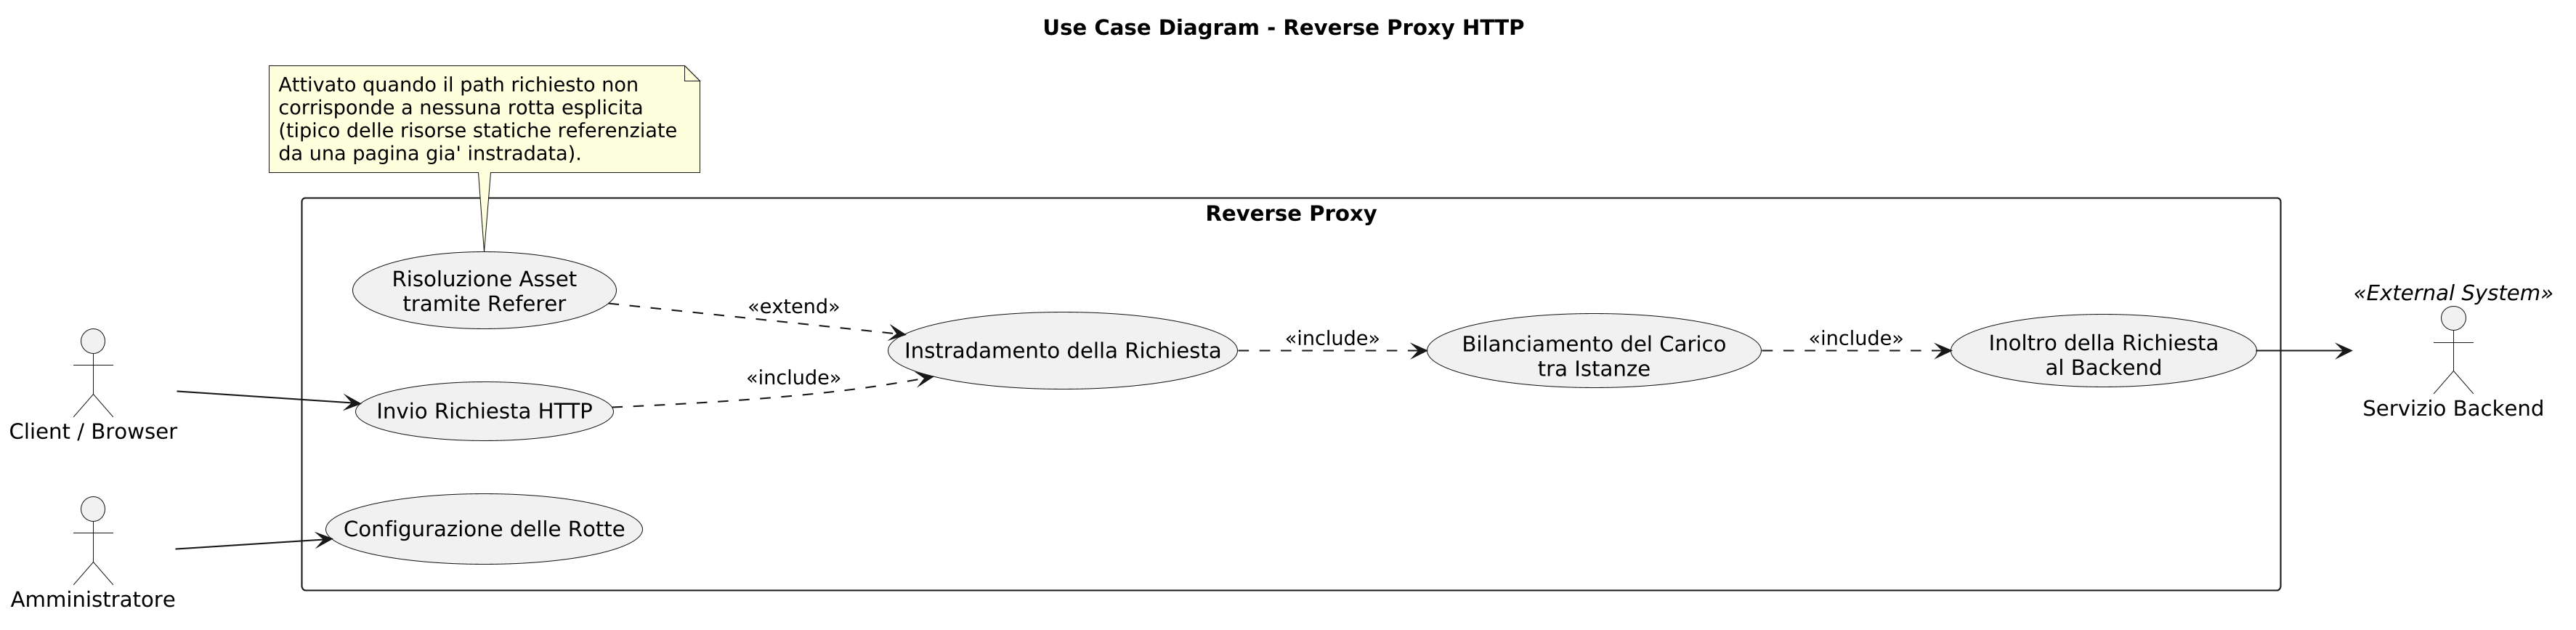
\includegraphics[width=\textwidth]{Images/uml/usecase.png}
    \caption{Use Case Diagram}
    \label{fig:usecase}
\end{figure}

\subsection{Class Diagram}

In questa sezione viene presentato il modello strutturale del sistema. \\
Le classi principali sono:

\begin{itemize}
    \item \textbf{ReverseProxy:} avvia il server e, per ogni connessione accettata, crea un nuovo \texttt{Client} a un pool di thread.
    \item \textbf{Client:} gestisce l'intero ciclo di vita di una singola connessione, dal parsing della richiesta fino alla chiusura dei socket.
    \item \textbf{HttpRequest:} rappresenta in maniera strutturata una richiesta HTTP, contenendo metodo, URL e header.
    \item \textbf{ConfigurationManager:} punto di accesso unico e globale alla configurazione caricata da file e alla strategia di balancing attiva.
    \item \textbf{Config, Route, Service:} il modello dati della configurazione creato direttamente dal file YAML. Una configurazione contiene più route, ciascuna delle quali può essere associata a uno o più servizi.
    \item \textbf{LoadBalancingStrategy e implementazioni:} l'interfaccia e le strategie concrete di selezione del servizio.
    \item \textbf{LoadBalancingStrategyFactory:} logica di creazione della strategia corretta.
\end{itemize}

\begin{figure}[H]
    \centering
    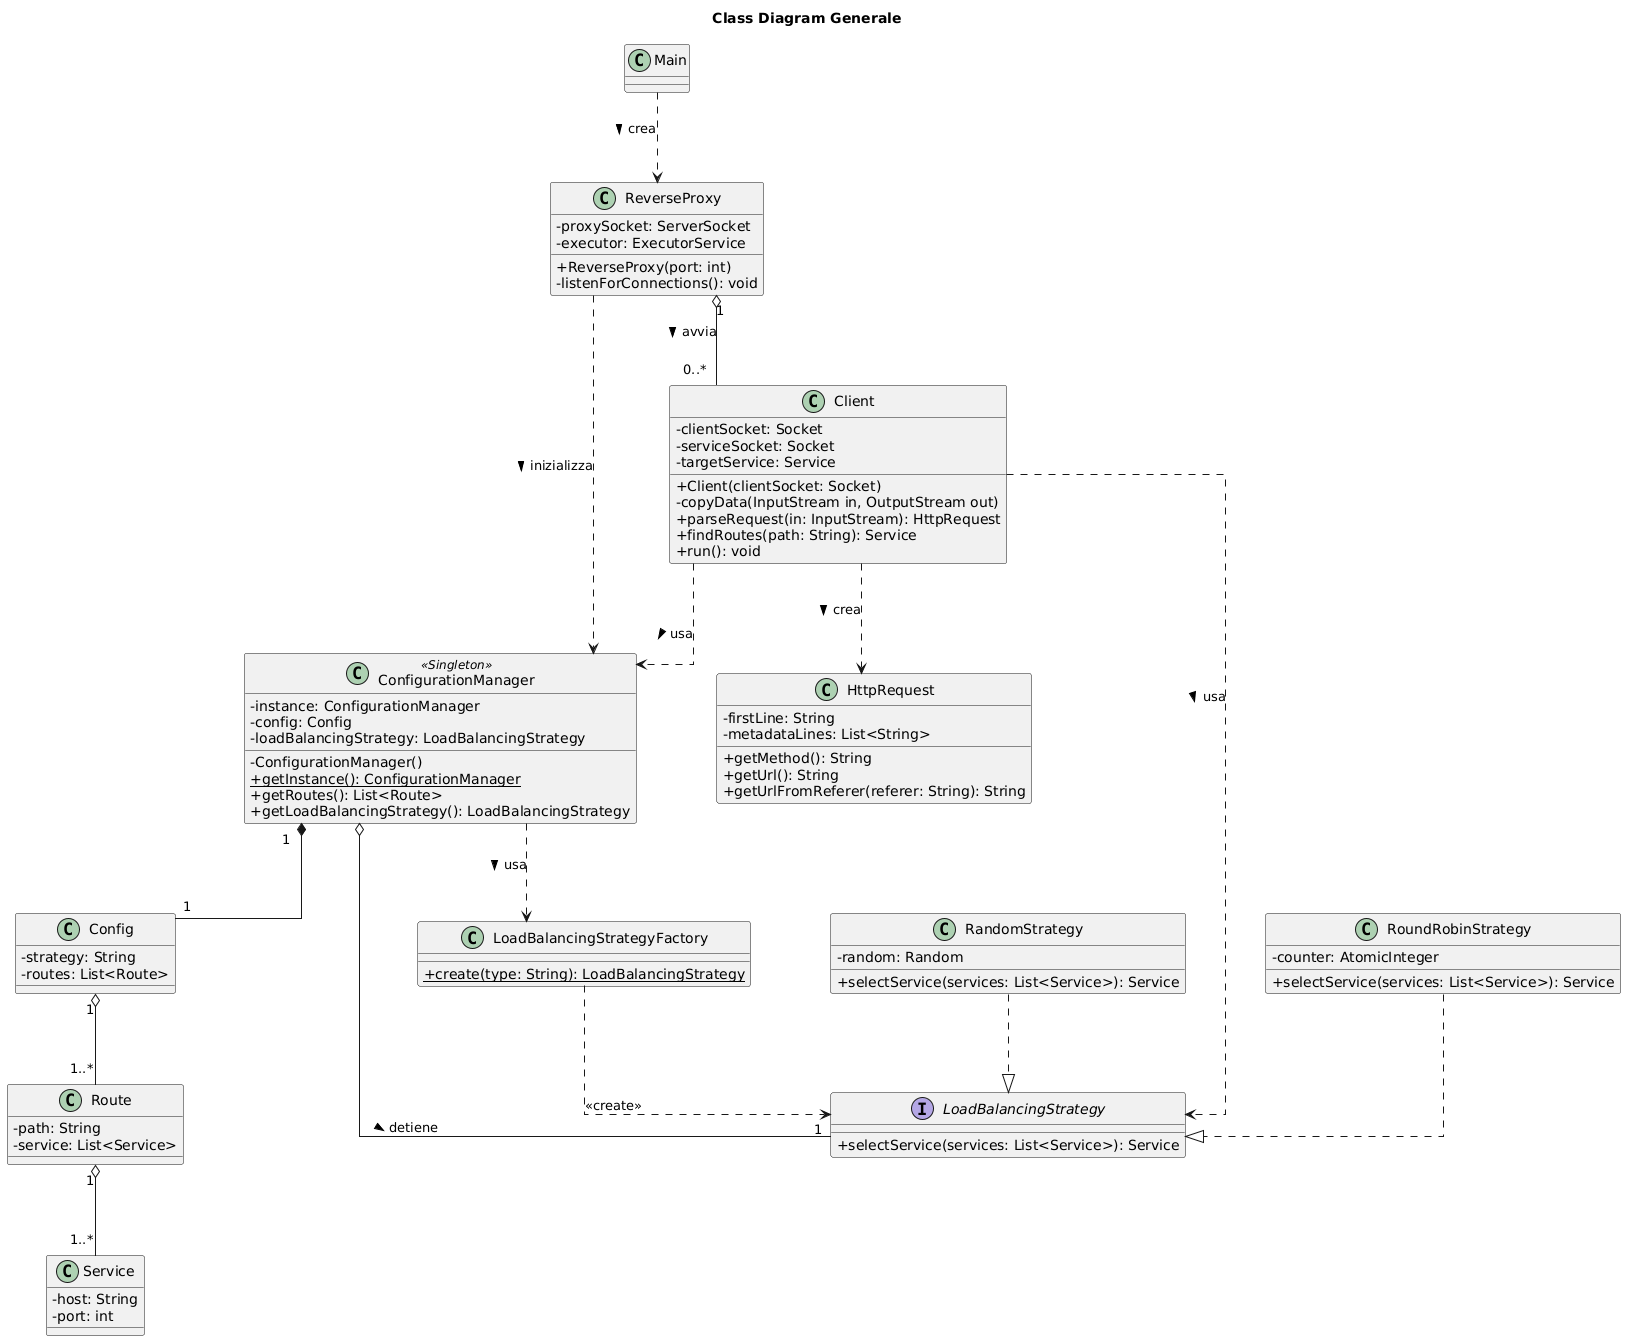
\includegraphics[width=\textwidth]{Images/uml/class.png}
    \caption{Class Diagram Generale}
    \label{fig:class}
\end{figure}

\subsection{Sequence Diagram}

Questo diagramma descrive lo scenario di inoltro di una richiesta verso una route con più istanze:

\begin{enumerate}
    \item Il client apre una connessione TCP e invia la richiesta HTTP.
    \item Il thread \texttt{Client} esegue il parsing della richiesta, ottenendo un oggetto \texttt{HttpRequest}.
    \item Vengono recuperate le route configurate tramite \texttt{ConfigurationManager}.
    \item Viene individuata la route corrispondente al percorso richiesto.
    \item Se la route esiste, viene presa la strategia di balacing e utilizzata per selezionare il servizio.
    \item Il thread \texttt{Client} apre una nuova connessione verso il servizio selezionato, inoltra la richiesta e poi la risposta ricevuta al client originario.
\end{enumerate}

La selezione dell'istanza di servizio è completamente delegata all'implementazione della strategia, mantenendo il \texttt{Client} indipendente dall'algoritmo utilizzato.

\begin{figure}[H]
    \centering
    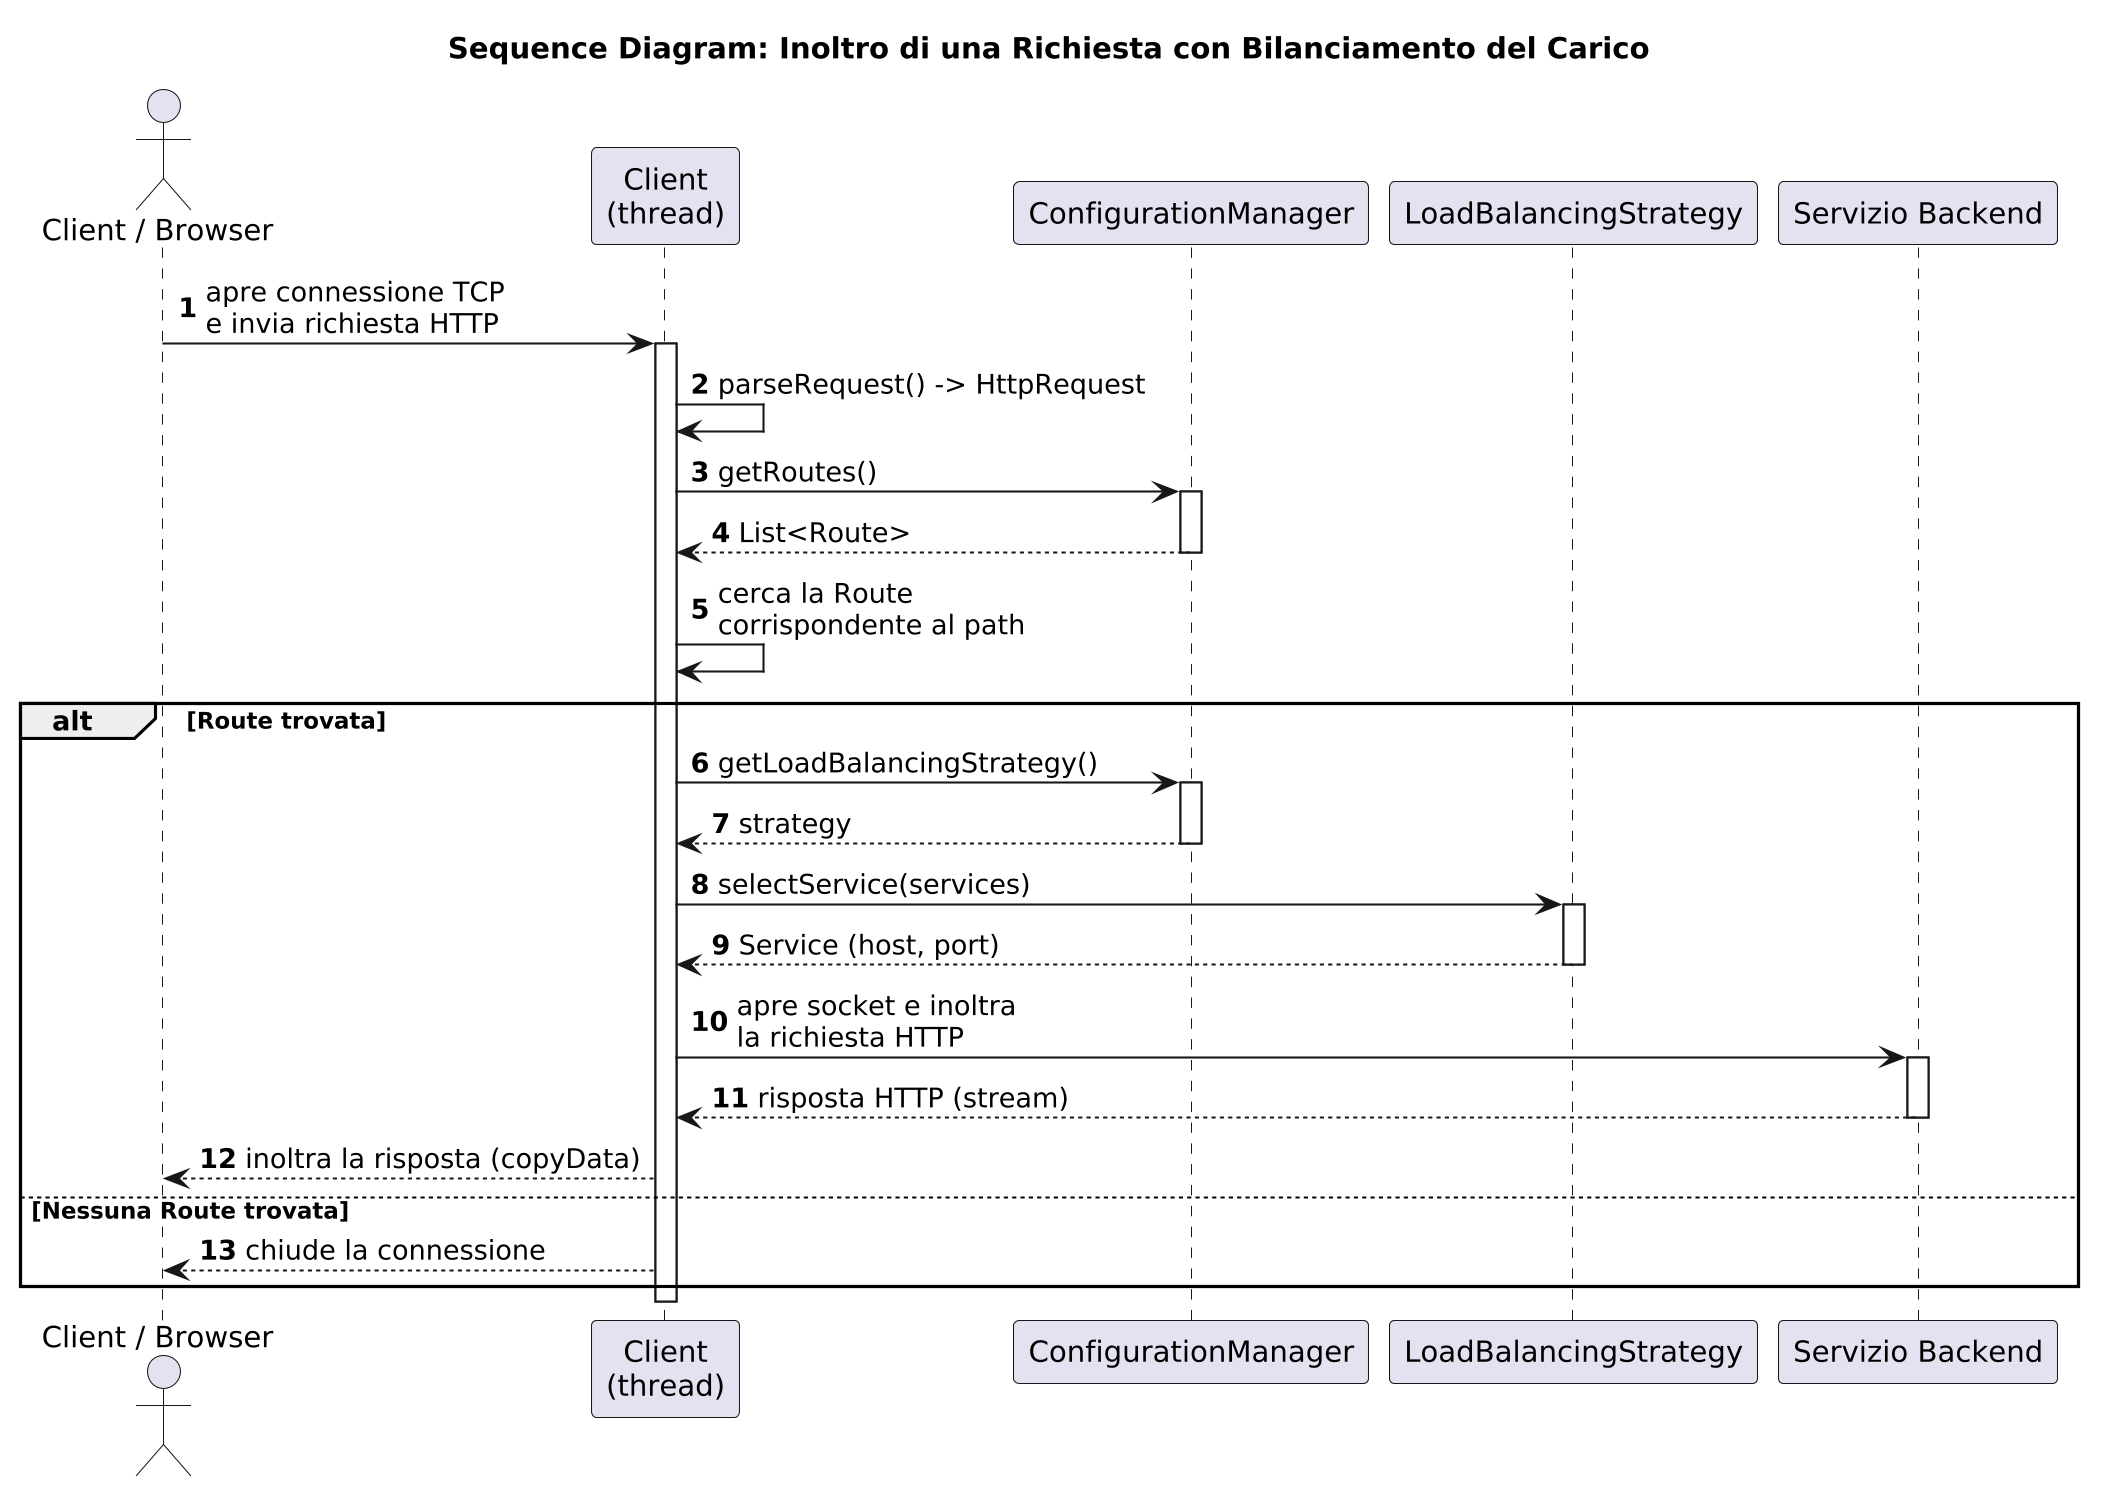
\includegraphics[width=\textwidth]{Images/uml/sequence.png}
    \caption{Sequence Diagram}
    \label{fig:sequence}
\end{figure}

\subsection{Activity Diagram}

Stesso scenario del diagramma precedente, ma rappresentato con un Activity Diagram.

\begin{figure}[H]
    \centering
    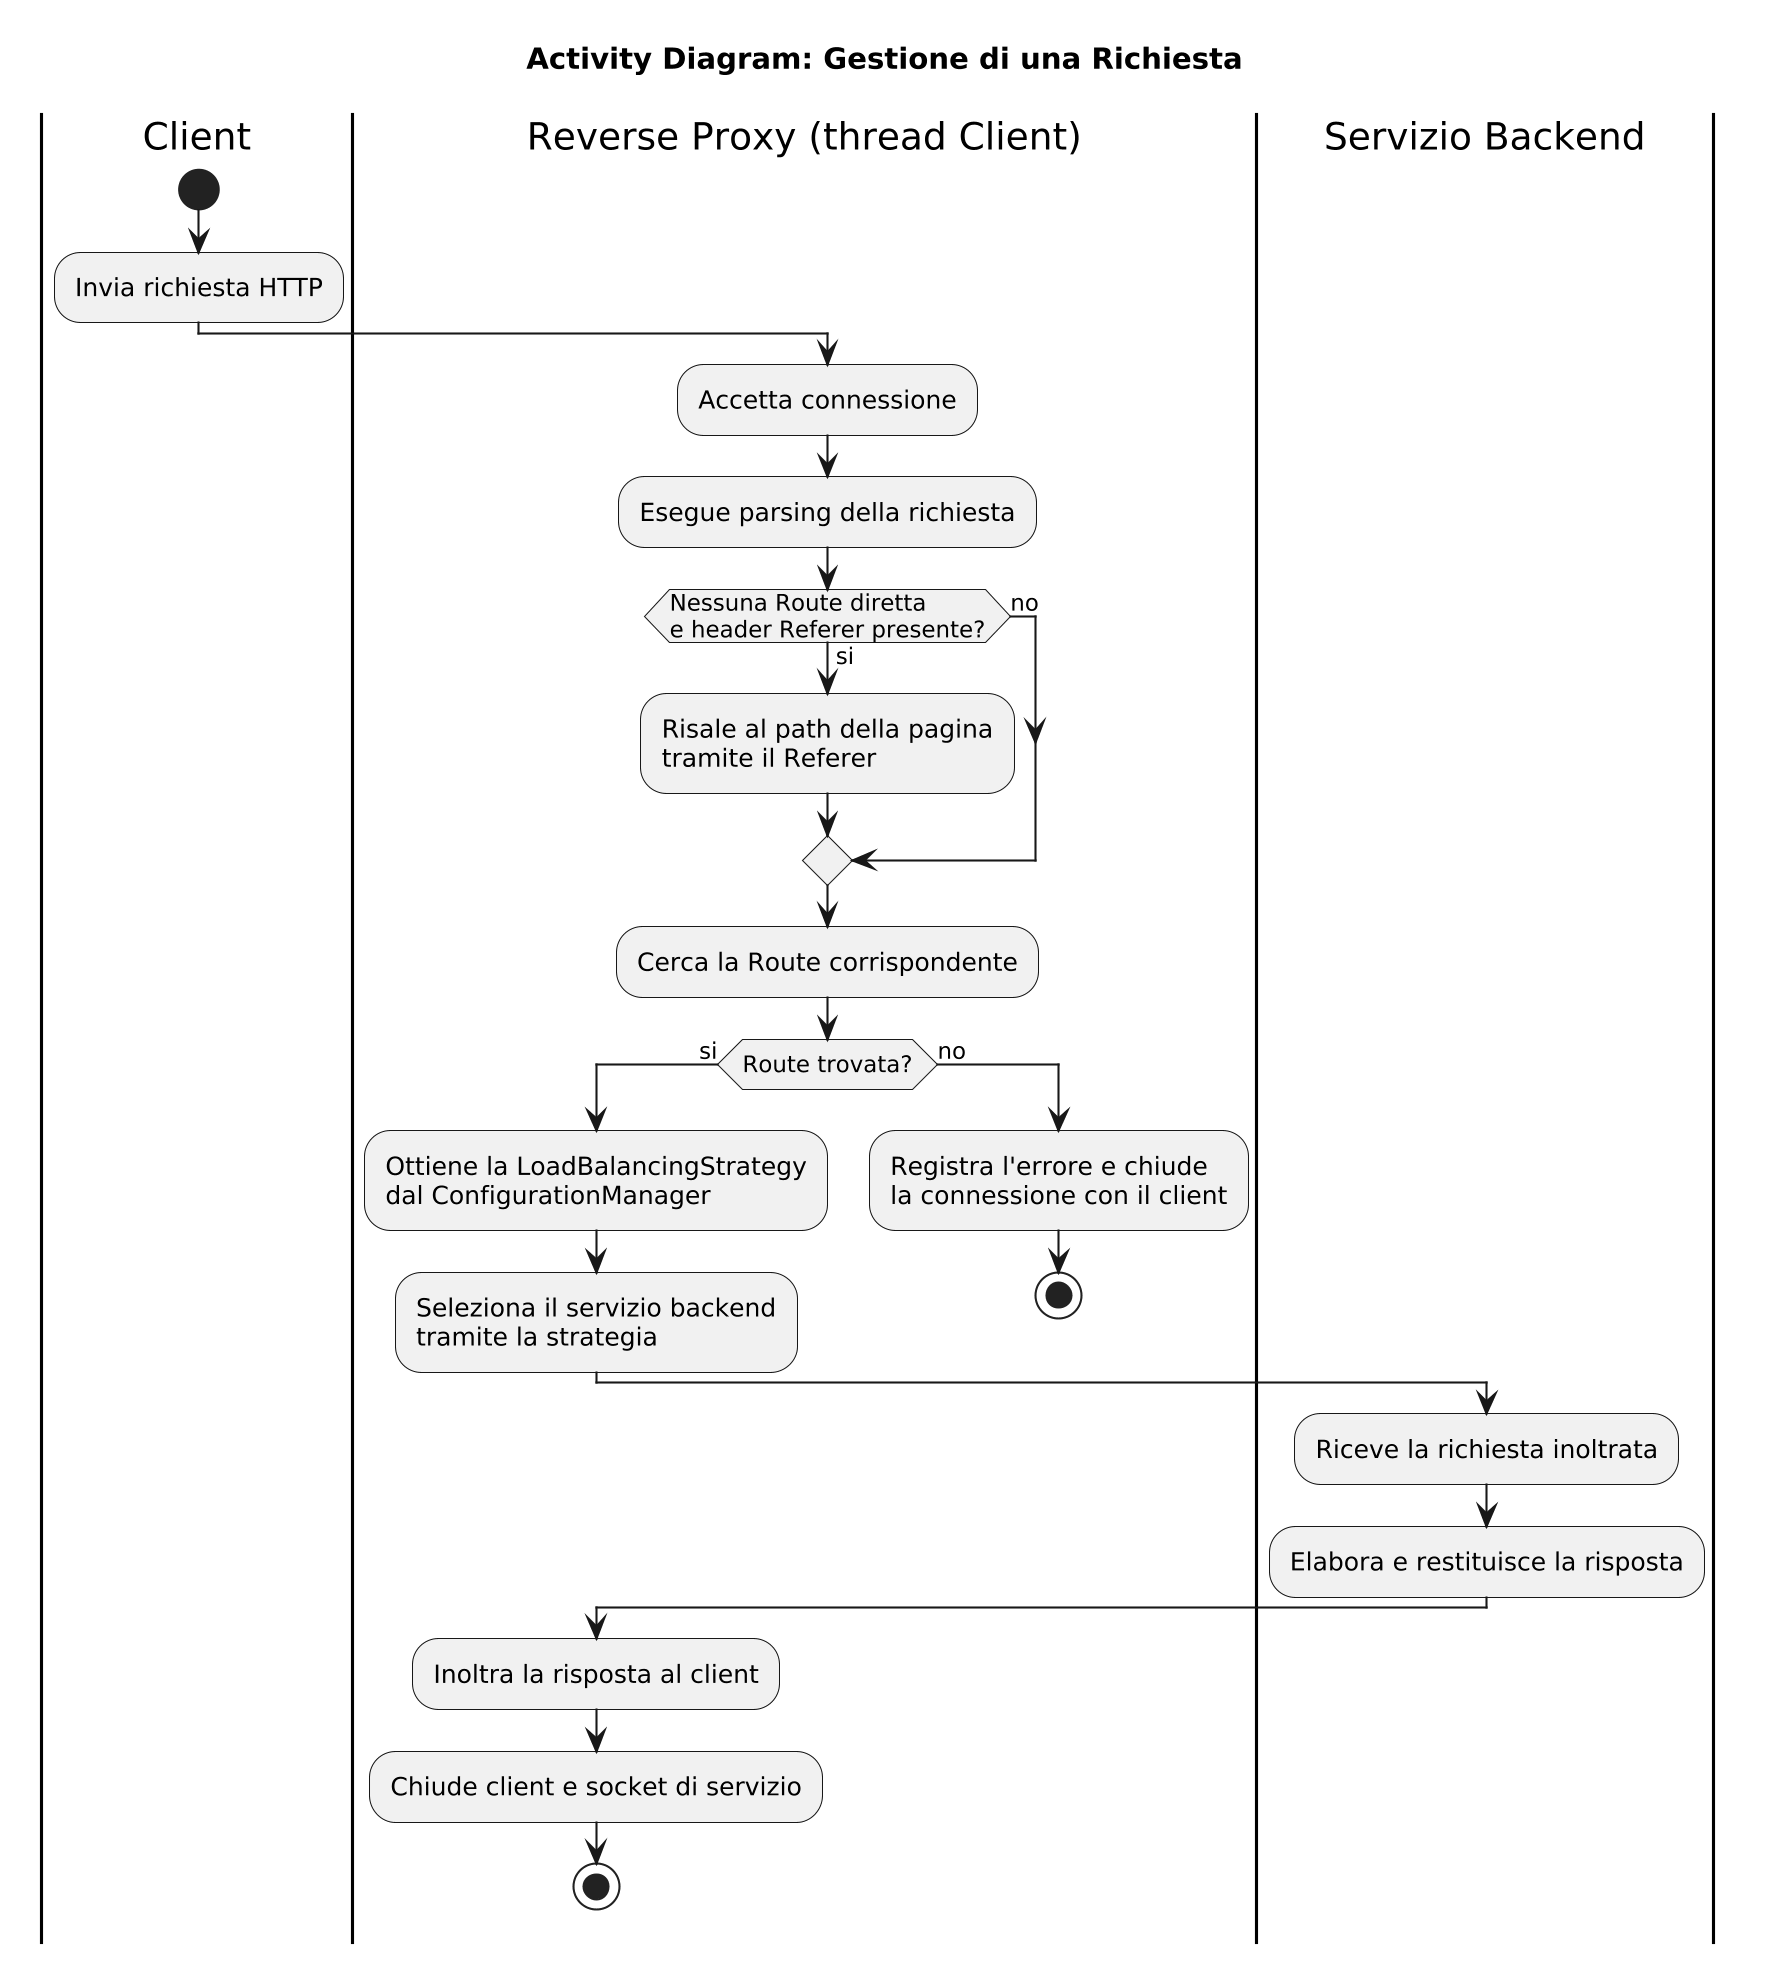
\includegraphics[width=0.78\textwidth]{Images/uml/activity.png}
    \caption{Activity Diagram}
    \label{fig:activity}
\end{figure}

\subsection{State Diagram}

Il diagramma descrive tutti gli stati di una connessione gestita da un thread \texttt{Client}.\\
Gli stati principali sono:

\begin{itemize}
    \item \textbf{Accettata:} stato iniziale, subito dopo l'accettazione della connessione da parte del \texttt{ServerSocket}.
    \item \textbf{InParsing:} la richiesta HTTP viene letta e trasformata in un oggetto \texttt{HttpRequest}.
    \item \textbf{InInstradamento:} viene ricercata la rotta corrispondente al percorso richiesto.
    \item \textbf{ConnessaAlBackend / InInoltro:} la connessione verso il servizio selezionato è stata aperta e la richiesta, poi la risposta, vengono inoltrate.
    \item \textbf{Fallita:} raggiunto in seguito a un errore di I/O o all'assenza di una route corrispondente.
    \item \textbf{Chiusa:} stato finale, raggiunto in ogni caso dal blocco \texttt{finally}, che garantisce il rilascio dei socket aperti indipendentemente dal risultato della richiesta.
\end{itemize}

\begin{figure}[H]
    \centering
    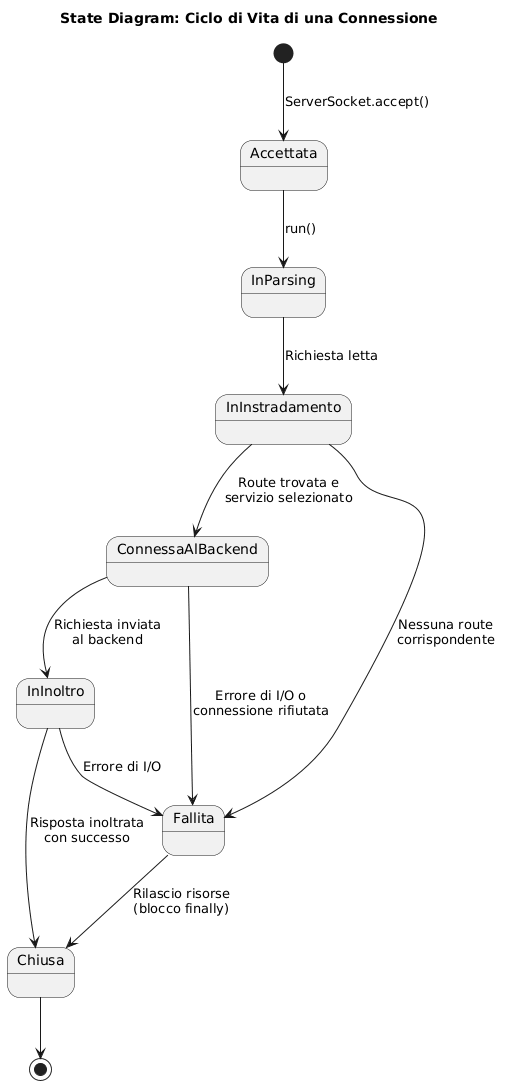
\includegraphics[width=0.5\textwidth]{Images/uml/state.png}
    \caption{State Diagram per una Connessione}
    \label{fig:state}
\end{figure}
